\documentclass[11pt,a4paper]{article}

% ----- preamble.tex -----
% % ----- preamble.tex -----
% % ----- preamble.tex -----
% \input{preamble.tex} should be included in all note files before '\begin{document}'
% \lecture{<lectureNumber>: <lectureTopic>}{<mm/dd/yyyy>}{<lecturerName>}{<authorName>}

\hbadness=10000
\vbadness=10000

% page size settings
\setlength{\textheight}{8.5in}
\setlength{\textwidth}{6.0in}
\setlength{\headheight}{0in}
\addtolength{\topmargin}{-.5in}
\addtolength{\oddsidemargin}{-.5in}

% paragraph spacing/indenting settings
\setlength\parindent{0pt}
\setlength\parskip{2.5pt}

% imported packages
\usepackage{amsmath,amssymb,amsthm}
\usepackage{mdframed} % for boxing
\usepackage{graphicx} % for inserting images
\graphicspath{ {./imgs/} }

\usepackage{diagbox} % backslash for tabular/tables
\usepackage{booktabs} % enhances quality of table presentation
\usepackage{tikz}
\usetikzlibrary{arrows,automata,trees,calc}

% ----- \tableofcontents PAGE LINKING (without blue highlight) -----
\usepackage{hyperref}
\hypersetup{
    colorlinks,
    citecolor=black,
    filecolor=black,
    linkcolor=black,
    urlcolor=black
}

% ----- VARIABLE RE-DEFINITIONS -----
\def\epsilon{\varepsilon}
\def\phi{\varphi}


% ----- TODO: MAKE EVERY NEW SECTION START ON NEW PAGE EXCLUDING TOC -----
% \let\oldsection\section
% \renewcommand{\section}{\newpage\oldsection}


% ----- CUSTOM COMMANDS -----
\newcommand{\handout}[5]{
    % \renewcommand{\thepage}{#1-\arabic{page}}
    \noindent
    \begin{center}
        \framebox{
            \vbox{
                \hbox to 5.78in {{\bf CS 4510: Automata and Complexity}\hfill #2}
                \vspace{4mm}
                \hbox to 5.78in {{\Large \hfill #5  \hfill}}
                \vspace{2mm}
                \hbox to 5.78in {{\it #3 \hfill #4}}
            }
        }
   \end{center}
   \vspace*{4mm}
}

\newcommand{\lecture}[4]{\handout{#1}{#2}{Lecturer: #3}{Author: #4}{Lecture #1}}

% keeps contents of the same theorem on the same page
\newcommand{\blocktheorem}[1]{
    \csletcs{old#1}{#1}
    \csletcs{endold#1}{end#1}
    \RenewDocumentEnvironment{#1}{o}{
        % \par\addvspace{cm}
        \noindent\begin{minipage}{\textwidth}
        \IfNoValueTF{##1}{\csuse{old#1}}{\csuse{old#1}[##1]}}{\csuse{endold#1}
        \end{minipage}
        \par\addvspace{0.75cm}
    }
}
\raggedbottom

\theoremstyle{definition}
\newtheorem{example}{Example} % use for example problems
\newmdtheoremenv{definition}{Definition} % use for definitions
\newtheorem{theorem}{Theorem} % use for theorems
\newtheorem{corollary}{Corollary} % use for corollary
\newtheorem{lemma}{Lemma} % use for corollary
\newtheorem{claim}{Claim}

\blocktheorem{example}
\blocktheorem{definition}
\blocktheorem{theorem}
\blocktheorem{corollary}
\blocktheorem{lemma}
\blocktheorem{claim} should be included in all note files before '\begin{document}'
% \lecture{<lectureNumber>: <lectureTopic>}{<mm/dd/yyyy>}{<lecturerName>}{<authorName>}

\hbadness=10000
\vbadness=10000

% page size settings
\setlength{\textheight}{8.5in}
\setlength{\textwidth}{6.0in}
\setlength{\headheight}{0in}
\addtolength{\topmargin}{-.5in}
\addtolength{\oddsidemargin}{-.5in}

% paragraph spacing/indenting settings
\setlength\parindent{0pt}
\setlength\parskip{2.5pt}

% imported packages
\usepackage{amsmath,amssymb,amsthm}
\usepackage{mdframed} % for boxing
\usepackage{graphicx} % for inserting images
\graphicspath{ {./imgs/} }

\usepackage{diagbox} % backslash for tabular/tables
\usepackage{booktabs} % enhances quality of table presentation
\usepackage{tikz}
\usetikzlibrary{arrows,automata,trees,calc}

% ----- \tableofcontents PAGE LINKING (without blue highlight) -----
\usepackage{hyperref}
\hypersetup{
    colorlinks,
    citecolor=black,
    filecolor=black,
    linkcolor=black,
    urlcolor=black
}

% ----- VARIABLE RE-DEFINITIONS -----
\def\epsilon{\varepsilon}
\def\phi{\varphi}


% ----- TODO: MAKE EVERY NEW SECTION START ON NEW PAGE EXCLUDING TOC -----
% \let\oldsection\section
% \renewcommand{\section}{\newpage\oldsection}


% ----- CUSTOM COMMANDS -----
\newcommand{\handout}[5]{
    % \renewcommand{\thepage}{#1-\arabic{page}}
    \noindent
    \begin{center}
        \framebox{
            \vbox{
                \hbox to 5.78in {{\bf CS 4510: Automata and Complexity}\hfill #2}
                \vspace{4mm}
                \hbox to 5.78in {{\Large \hfill #5  \hfill}}
                \vspace{2mm}
                \hbox to 5.78in {{\it #3 \hfill #4}}
            }
        }
   \end{center}
   \vspace*{4mm}
}

\newcommand{\lecture}[4]{\handout{#1}{#2}{Lecturer: #3}{Author: #4}{Lecture #1}}

% keeps contents of the same theorem on the same page
\newcommand{\blocktheorem}[1]{
    \csletcs{old#1}{#1}
    \csletcs{endold#1}{end#1}
    \RenewDocumentEnvironment{#1}{o}{
        % \par\addvspace{cm}
        \noindent\begin{minipage}{\textwidth}
        \IfNoValueTF{##1}{\csuse{old#1}}{\csuse{old#1}[##1]}}{\csuse{endold#1}
        \end{minipage}
        \par\addvspace{0.75cm}
    }
}
\raggedbottom

\theoremstyle{definition}
\newtheorem{example}{Example} % use for example problems
\newmdtheoremenv{definition}{Definition} % use for definitions
\newtheorem{theorem}{Theorem} % use for theorems
\newtheorem{corollary}{Corollary} % use for corollary
\newtheorem{lemma}{Lemma} % use for corollary
\newtheorem{claim}{Claim}

\blocktheorem{example}
\blocktheorem{definition}
\blocktheorem{theorem}
\blocktheorem{corollary}
\blocktheorem{lemma}
\blocktheorem{claim} should be included in all note files before '\begin{document}'
% \lecture{<lectureNumber>: <lectureTopic>}{<mm/dd/yyyy>}{<lecturerName>}{<authorName>}

\hbadness=10000
\vbadness=10000

% page size settings
\setlength{\textheight}{8.5in}
\setlength{\textwidth}{6.0in}
\setlength{\headheight}{0in}
\addtolength{\topmargin}{-.5in}
\addtolength{\oddsidemargin}{-.5in}

% paragraph spacing/indenting settings
\setlength\parindent{0pt}
\setlength\parskip{2.5pt}

% imported packages
\usepackage{amsmath,amssymb,amsthm}
\usepackage{mdframed} % for boxing
\usepackage{graphicx} % for inserting images
\graphicspath{ {./imgs/} }

\usepackage{diagbox} % backslash for tabular/tables
\usepackage{booktabs} % enhances quality of table presentation
\usepackage{tikz}
\usetikzlibrary{arrows,automata,trees,calc}

% ----- \tableofcontents PAGE LINKING (without blue highlight) -----
\usepackage{hyperref}
\hypersetup{
    colorlinks,
    citecolor=black,
    filecolor=black,
    linkcolor=black,
    urlcolor=black
}

% ----- VARIABLE RE-DEFINITIONS -----
\def\epsilon{\varepsilon}
\def\phi{\varphi}


% ----- TODO: MAKE EVERY NEW SECTION START ON NEW PAGE EXCLUDING TOC -----
% \let\oldsection\section
% \renewcommand{\section}{\newpage\oldsection}


% ----- CUSTOM COMMANDS -----
\newcommand{\handout}[5]{
    % \renewcommand{\thepage}{#1-\arabic{page}}
    \noindent
    \begin{center}
        \framebox{
            \vbox{
                \hbox to 5.78in {{\bf CS 4510: Automata and Complexity}\hfill #2}
                \vspace{4mm}
                \hbox to 5.78in {{\Large \hfill #5  \hfill}}
                \vspace{2mm}
                \hbox to 5.78in {{\it #3 \hfill #4}}
            }
        }
   \end{center}
   \vspace*{4mm}
}

\newcommand{\lecture}[4]{\handout{#1}{#2}{Lecturer: #3}{Author: #4}{Lecture #1}}

% keeps contents of the same theorem on the same page
\newcommand{\blocktheorem}[1]{
    \csletcs{old#1}{#1}
    \csletcs{endold#1}{end#1}
    \RenewDocumentEnvironment{#1}{o}{
        % \par\addvspace{cm}
        \noindent\begin{minipage}{\textwidth}
        \IfNoValueTF{##1}{\csuse{old#1}}{\csuse{old#1}[##1]}}{\csuse{endold#1}
        \end{minipage}
        \par\addvspace{0.75cm}
    }
}
\raggedbottom

\theoremstyle{definition}
\newtheorem{example}{Example} % use for example problems
\newmdtheoremenv{definition}{Definition} % use for definitions
\newtheorem{theorem}{Theorem} % use for theorems
\newtheorem{corollary}{Corollary} % use for corollary
\newtheorem{lemma}{Lemma} % use for corollary
\newtheorem{claim}{Claim}

\blocktheorem{example}
\blocktheorem{definition}
\blocktheorem{theorem}
\blocktheorem{corollary}
\blocktheorem{lemma}
\blocktheorem{claim}

\begin{document}
\lecture{6: Regular Expressions}{09/08/2022}{Zvi Galil}{Austin Peng}
\tableofcontents

% TODO: how do i fix this to have new page before every section, but not before the table of contents
\AddToHook{cmd/section/before}{\newpage}

\section{Regular Expression vs. Arithmetic Expression}

We have seen two different ways to define regular languages: DFAs and NFAs. We
will introduce a third way, called a \textbf{regular expression (reg exp)}, that represent the same class of
language as DFAs and NFAs. \\

It is easiest to compare regular expressions to arithmetic expressions to explain them. Consider an arithmetic expression, such as (5+3)·42, which is applied over the integers.
Regular expressions are similar, but instead they operate on languages. Let us consider an example of a regular expression, such as $(0\cup 1)\circ 0^*$.
This regular expressions denotes a language that includes all string that start with a 0 or 1 and then followed by any number of zeros.
It is important to note here that we use $0$ as a shorthand for the set $\{0\}$, and the same with $1$ and the set $\{1\}$, since regular expressions operate over sets of strings (languages).
More examples of regular expressions we have already seen include $\Sigma^*$ and $(0\cup1)^*$.
Just how we often drop the multiplication operator when writing an arithmetic operation, we can also drop the concatenation operator when writing a regular expression.
For example, we can write the arithmetic expression above as $(5+3)\cdot4^2$, and the first regular expression can be written as $(0\cup 1)0^*$.
It is understood that the operations of multiplication, and concatenation, respectively are still present even if not explicitly written out.
In addition, there is a hierarchy of operator precedence in regular expressions just like in arithmetic expressions (PEMDAS). The order is:
\begin{enumerate}
    \item parenthesis $()$
    \item Kleene star $*$
    \item concatenation
    \item union
\end{enumerate}

\section{Formal Definition Of A Regular Expression}
\begin{definition}
    Say that $R$ is a regular expression if $R$ is:
    \begin{enumerate}
        \item $a$ for some $a$ in the alphabet $\Sigma$
        \item $\epsilon$
        \item $\emptyset$
        \item $(R_1\cup R_2)$, where $R_1$ and $R_2$ are regular expressions
        \item $(R_1\circ R_2)$, where $R_1$ and $R_2$ are regular expressions
        \item $(R_1)^*$, where $R_1$ is a regular expression
    \end{enumerate}

    In items $1$ and $2$, the regular expressions $a$ and $\epsilon$ represent the languages $\{a\}$ and $\{\epsilon\}$, respectively. \\

    In item 3, the regular expression $\emptyset$ represents the empty language. \\

    In item $4,5,$ and $6$, the expressions represent the languages obtained by taking the union or concatenation of the languages $R_1$ and $R_2$, or the star of the languages $R_1$, respectively. \\
\end{definition}

\section{Examples: Regular Expressions}
\begin{example}
    Consider the regular expression: $0^*10^*$ \\
    
    It represents all binary strings that contains exactly one $1$. This includes strings like $0010000000$, $1000$, and $1$.
\end{example}

\begin{example}
    Consider the regular expression: $\Sigma^* abracadabra\Sigma^*$ \\

    It represents all strings that contain the substring $abracadabra$.
\end{example}

\begin{example}
    Consider the regular expression $(\Sigma\Sigma)^*$ \\

    It represents all strings of even length.
\end{example}


\section{Identities}
\begin{itemize}
    \item $\emptyset^*=\{\epsilon\}$ since the Kleene star operator always contains the empty string.
    \item $1^*\emptyset=\emptyset$ since some number of $1$s followed by an element from the empty set cannot exist
    \item $R\cup\emptyset=R$
    \item $R\circ\epsilon=R$
    \item Note that $R\cup\epsilon$ is only equal to $R$ if $R$ contains $\epsilon$
    \item $R\emptyset=\emptyset$
\end{itemize}

\section{Formal Definition Of A Generalized Nondeterministic Finite Automata}
For convenience, GNFAs always have a special form that meets the following conditions:
\begin{itemize}
    \item The start state has transition arrows going to every other state but no arrows coming in from any other state.
    \item There is only a single accepting state, and it has arrows coming in from every other state but no arrows going to any other state. The accepting state is not the same as the start state.
    \item Except for the start and accepting states, one arrow goes from every state to every other state and also from each state to itself.
\end{itemize}

The following idea is used for the proof later:

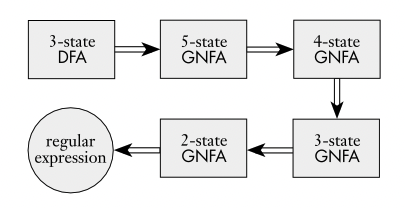
\includegraphics[width=\linewidth / 2]{lecture06-idea-convert-dfa-to-reg-exp.png}

If the $GNFA$ has $k$ states, then we know that $k\geq 2$ since a GNFA must have a start and accepting state that must be different from each other. \\

If $k>2$, we construct an equivalent $GNFA$ with $k-1$ states. This step can be repeated on the new $GNFA$ until it is reduced to 2 states. \\

If $k=2$, the GNFA has a single arrow that goes from the start state to the accepting state. The label of this arrow is the equivalent regular expression. \\

The important step is constructing an equivalent GNFA with 1 fewer state when $k>2$.
This is done by selecting a state $q_{rip}$ and "ripping" it out of the machine, and repairing the remainder so that the same language is still recognized.
Any state works, as long as it is not the start or accepting state. \\

After removing $q_{rip}$, the machine is repaired by altering the regular expressions that label each of the remaining arrows.
The new labels compensate for the absence of $q_{rip}$. THe new label going from $q_i$ to $q_j$ is a regular expression that describes all strings that would take the machine from $q_i$ to $q_j$ either directly or through $q_{rip}$.

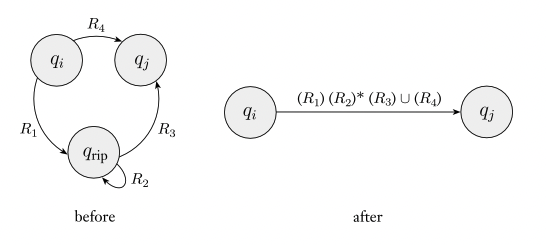
\includegraphics[width=\linewidth * 2 / 3]{lecture06-handling-q-rip.png} \\

\begin{example}
    Constructing an equivalent GNFA with one fewer state. \\

    In the old machine, if
    \begin{itemize}
        \item $q_i$ goes to $q_{rip}$ with an arrow labeled $R_1$
        \item $q_{rip}$ goes to itself with an arrow labeled $R_2$
        \item $q{rip}$ goes to $q_j$ with an arrow labeled $R_3$
        \item $q_i$ goes to $q_j$ with an arrow labeled $R_4$
    \end{itemize}
    then in the new machine, the arrow from $q_i$ to $q_j$ gets the label $$(R_1)(R_2)^*(R_3)\cup(R_4)$$
\end{example}

\begin{definition}
    A generalized nondeterministic finite automaton is a 5-tuple, $(Q,\Sigma,\delta, q_{start}, q_{accept})$, where:
    \begin{enumerate}
        \item $Q$ is the finite set of states
        \item $\Sigma$ is the input alphabet
        \item $\delta:(Q-\{q_{accept}\})\times(Q-\{q_{start}\})\rightarrow\mathcal{R}$ is the transition function
        \item $q_{start}$ is the start state
        \item $q_{accept}$ is the accepting state
    \end{enumerate}
\end{definition}

A GNFA accepts a string $w$ in $\Sigma^*$ if $w=w_1w_2...w_k$, where each $w_i$ is in the $\Sigma^*$ and a sequence of states $q_0,q_1,...,q_k$ exists such that
\begin{itemize}
    \item $q_0=q_{start}$ is the start state
    \item $q_k=q_{accept}$ is the accepting state
    \item for each $i$, we have $w_i\in L(R_i)$, where $R_i=\delta(q_{i-1},q_i)$ (aka $R_i$ is the expression on the arrow from $q_{i-1}$ to $q_i$)
\end{itemize}

\subsection{Langauge Is Regular IFF Some Regular Expression Describes It}
\begin{theorem}
    A language is regular if an only if some regular expression describes it.

    \begin{proof}
        The proof has two directions, and we will prove both directions as separate lemmas.
    \end{proof}
\end{theorem}

\begin{lemma}
    If a language is described by a regular expression, then it is regular.

    \begin{proof}
        Let us convert $R$ into an NFA $N$. We consider the 6 cases in the formal definition of regular expression.
        \begin{enumerate}
            \item $R=a$ for some $a\in\Sigma$. Then $L(R)=\{a\}$, and the following NFA recognizes $L(R)$. \\
            
            \begin{tikzpicture}[node distance={2cm}, semithick, main/.style = {draw, circle}]
                \node[name=input] {};
                \node[state] (0) [right of=input] {};
                \node[state,accepting] (1) [right of=0] {};
        
                \draw[->] (input) -- (0);
                \draw[->] (0) to node[above] {$a$} (1);
            \end{tikzpicture} \\

            Note that this machine fits the definition of NFA but not DFA (but we can provide an equivalent DFA).

            \item $R=\epsilon$. Then $L(R)=\{\epsilon\}$, and the following NFA recognizes $L(R)$. \\
            
            \begin{tikzpicture}[node distance={2cm}, semithick, main/.style = {draw, circle}]
                \node[name=input] {};
                \node[state,accepting] (0) [right of=input] {};
        
                \draw[->] (input) -- (0);
            \end{tikzpicture} \\

            \item $R=\emptyset$. Then $L(R)=\emptyset$, and the following NFA recognizes $L(R)$. \\
            
            \begin{tikzpicture}[node distance={2cm}, semithick, main/.style = {draw, circle}]
                \node[name=input] {};
                \node[state] (0) [right of=input] {};
        
                \draw[->] (input) -- (0);
            \end{tikzpicture} \\
            
            \item $R=R_1\cup R_2$
            \item $R=R_1\circ R_2$
            \item $R=R_1^*$
        \end{enumerate}

        Note that for items 4-6, we use the constructions given in the proofs that the class of regular languages is closed under the regular operations. \\
    \end{proof}
\end{lemma}



\begin{lemma}
    If a language is regular, then it is described by a regular expression. \\

    \textit{Proof Idea.} We need to show that if a language $A$ is regular, a regular expression describes it.
    Because $A$ is regular, it is accepted by a DFA, which we can convert into an equivalent regular expression. \\

    First we show how to convert DFAs into generalized nondeterministic finite automatons (GNFAs), and then GNFAs into regular expressions.

    \begin{proof}
        Let $M$ be the DFA for the language $A$. Then we convert $M$ to a GNFA $G$ by adding a new start state, a new accepting state, and additional transition arrows as needed.
        Let the proecedure $CONVERT(G)$ which takes a GNFA and returns an equivalent regular expression (using recursion where each call to itself processes a GNFA with 1 fewer state). \\

        $CONVERT(G)$
        \begin{enumerate}
            \item Let $k$ be the number of states of $G$.
            \item If $k=2$, then $G$ must consist of a start state, an accepting state, and a single arrow connecting them and labeled with a regular expression $R$. Return the expression $R$.
            \item If $k>2$, we select any state $q_{rip}\in Q$ different from $q_{start}$ and $q_{accept}$ and let $G'$ be the GNFA $(Q',\Sigma,\delta',q_{start},q_{accept})$, where
            $$Q'=Q-\{q_{rip}\},$$
            and for any $q_i\in Q'-\{q_{accept}\}$ and any $q_j\in Q'-\{q_{start}\}$, let
            $$\delta'(q_i,q_j)=(R_1)(R_2)^*(R_3)\cup(R_4),$$
            for $R_1=\delta(q_i,q_{rip}),R_2=\delta(q_{rip},q_{rip}),R_3=\delta(q_{rip},q_j),R_4=\delta(q_i,q_j)$.
            \item Compute $CONVERT(G')$ and return this value.
        \end{enumerate}
    \end{proof}
\end{lemma}

\begin{claim}
    For any GNFA $G$, $CONVERT(G)$ is equivalent to $G$. \\

    \begin{proof}
        We will prove this claim using induction. \\

        Basis: Prove the claim is true for $k=2$ states.

        If $G$ has only 2 states, it can have only a single arrow going from start to accepting.
        The regular expression label on this arrow describes all the st rings that allow $G$ to get to the accepting state.
        Therefore, it is equivalent to $G$. \\

        Induction step: Assume that the claim is true for $k-1$ states and use this assumption to prove that the claim is true for $k$ states.

        First show that $G$ and $G'$ recognize the same language. Suppose that $G$ accepts input $w$. Then in an accepting branch of computation, $G$ enters a sequence of states: $$q_{start},q_1,q_2,\cdots,q_{accept}$$
        If none of them is the removed state $q_{rip}$, then $G'$ accepts $w$. This is because $G'$ contains the old regular expression as part of a union. \\

        If $q_{rip}$ appears, removing each run of consecutive $q_{rip}$ states forms an accepting computation for $G'$.
        This is because the states $q_i$ and $q_j$ now have a new regular expression on the arrow between them that describes all strings taking $q_i$ to $q_j$ through $q_{rip}$ on $G$. So $G'$ accepts $w$. \\

        Suppose that $G'$ accepts an input $w$. Since each arrow between any 2 states $q_i$ and $q_j$ in $G'$ describes the collection of strings taking $q_i$ to $q_j$ in $G$, either directly or through $q_{rip}$, $G$ must also accept $w$.
    \end{proof}

\end{claim}
\end{document}